% -*- mode: latex; mode: flyspell; ispell-local-dictionary: "en_US"; coding: utf-8; fill-column: 80 -*-

\documentclass{article}

\usepackage[utf8]{inputenc}
\usepackage[english]{babel}

\usepackage{amsmath,amsfonts,amssymb}
\usepackage{fullpage}
\usepackage{verbatim}

\usepackage{tikz,pgfplots}

\pgfplotsset{
  width=150mm,height=100mm,
  major grid style={thin,dotted,color=black!50},
  minor grid style={thin,dotted,color=black!50},
  grid,
  every axis/.append style={
    line width=0.5pt,
    tick style={
      line cap=round,
      thin,
      major tick length=4pt,
      minor tick length=2pt,
    },
  },
  legend cell align=left,
  legend pos=north west,
}

%%%%%%%%%%%%%%%%%%%%%%%%%%%%%%%%%%%%%%%%%%%%%%%%%%%%%%%%%%%%%%%%%%%%%%%%%%%%%%%%

\begin{document}

\title{Speicherplatzanalyse Hashmaps}
\author{}
\maketitle


% IMPORT-DATA mphf stats_mphf_size.txt
% IMPORT-DATA change smaller_tables.txt
% IMPORT-DATA hashmap stats_hashmap_size.txt


\begin{center}
	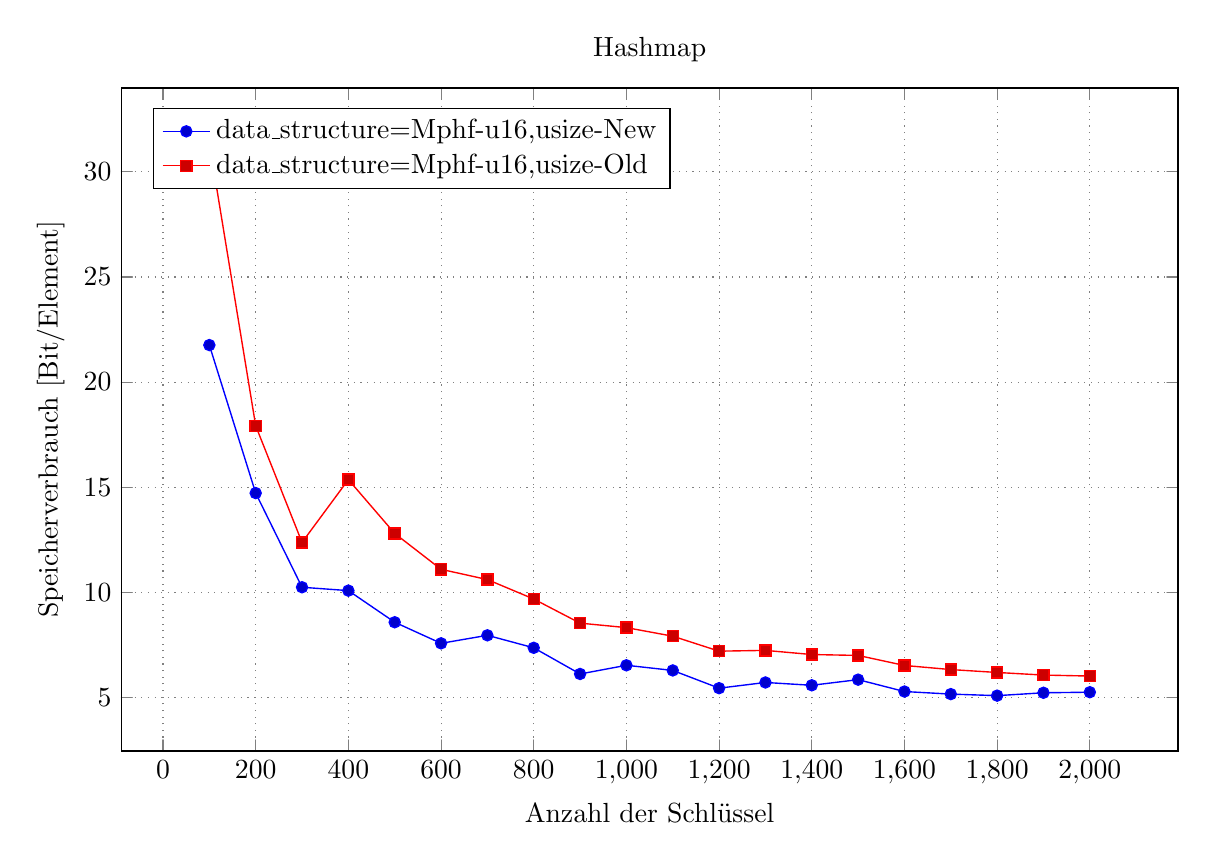
\begin{tikzpicture}
	\begin{axis}[
	title={Hashmap},
	xlabel={Anzahl der Schlüssel},
	ylabel={Speicherverbrauch [Bit/Element]},
	]
	
	%% MULTIPLOT(data_structure) SELECT size AS x, size_bytes AS y, MULTIPLOT
	%% FROM change WHERE x % 100 == 0 and x > 10 GROUP BY MULTIPLOT,x ORDER BY MULTIPLOT,x
 \addplot coordinates { (100,21.76) (200,14.72) (300,10.24) (400,10.08) (500,8.576) (600,7.57333) (700,7.95429) (800,7.36) (900,6.11556) (1000,6.528) (1100,6.28364) (1200,5.44) (1300,5.71077) (1400,5.57714) (1500,5.84533) (1600,5.28) (1700,5.15765) (1800,5.08444) (1900,5.22105) (2000,5.248) };
 \addlegendentry{data\_structure=Mphf-u16,usize-New};
 \addplot coordinates { (100,31.36) (200,17.92) (300,12.3733) (400,15.36) (500,12.8) (600,11.0933) (700,10.6057) (800,9.68) (900,8.53333) (1000,8.32) (1100,7.91273) (1200,7.2) (1300,7.23692) (1400,7.04) (1500,6.99733) (1600,6.52) (1700,6.32471) (1800,6.18667) (1900,6.06316) (2000,6.016) };
 \addlegendentry{data\_structure=Mphf-u16,usize-Old};
	
	
	
	
	
	\end{axis}
	\end{tikzpicture}
\end{center}

\begin{center}
	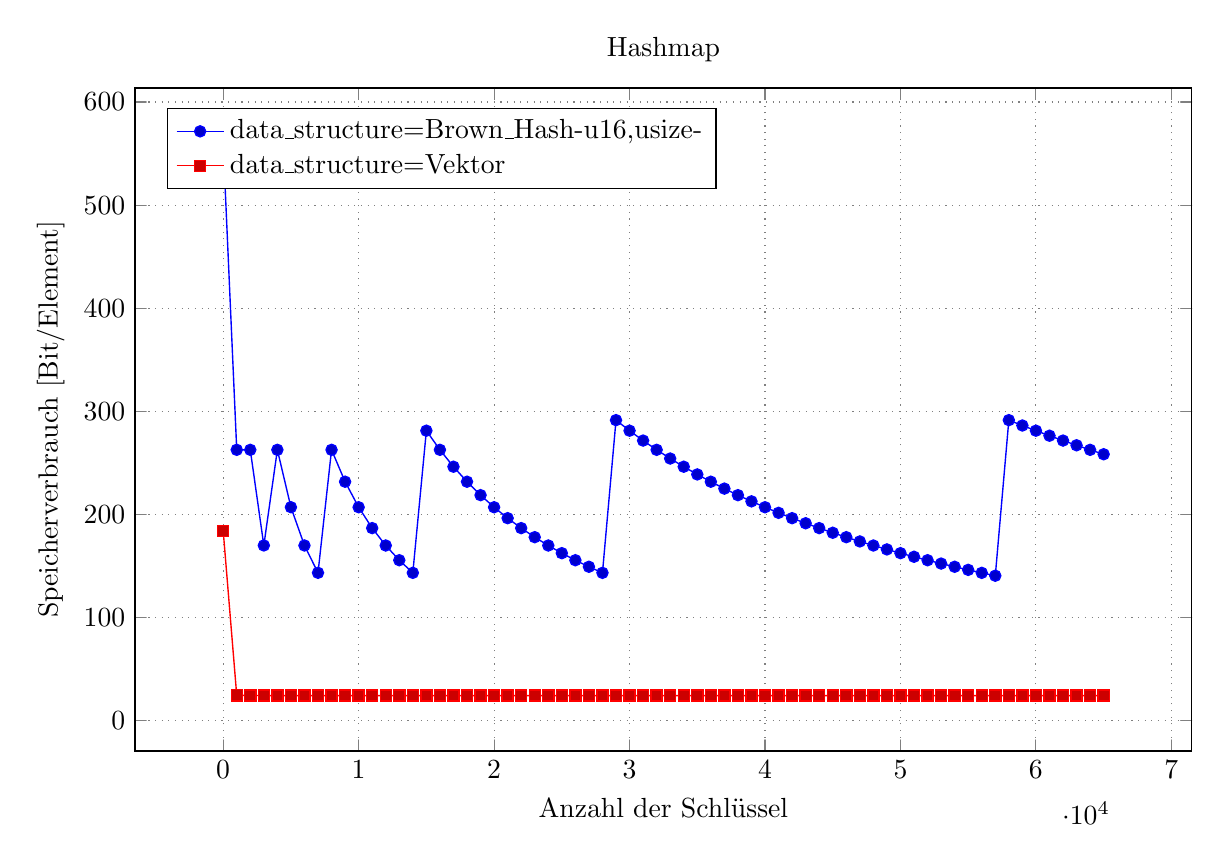
\begin{tikzpicture}
	\begin{axis}[
	title={Hashmap},
	xlabel={Anzahl der Schlüssel},
	ylabel={Speicherverbrauch [Bit/Element]},
	]
	
	%% MULTIPLOT(data_structure) SELECT size AS x, size_bytes AS y, MULTIPLOT
	%% FROM hashmap WHERE x % 1000 == 2  GROUP BY MULTIPLOT,x ORDER BY MULTIPLOT,x
 \addplot coordinates { (2,560.0) (1002,262.547) (2002,262.537) (3002,169.753) (4002,262.533) (5002,206.848) (6002,169.719) (7002,143.196) (8002,262.53) (9002,231.589) (10002,206.835) (11002,186.581) (12002,169.702) (13002,155.42) (14002,143.177) (15002,281.095) (16002,262.529) (17002,246.147) (18002,231.585) (19002,218.556) (20002,206.829) (21002,196.219) (22002,186.574) (23002,177.767) (24002,169.694) (25002,162.267) (26002,155.411) (27002,149.063) (28002,143.168) (29002,291.34) (30002,281.096) (31002,271.513) (32002,262.529) (33002,254.089) (34002,246.146) (35002,238.656) (36002,231.583) (37002,224.892) (38002,218.553) (39002,212.539) (40002,206.826) (41002,201.391) (42002,196.215) (43002,191.28) (44002,186.57) (45002,182.068) (46002,177.763) (47002,173.64) (48002,169.69) (49002,165.9) (50002,162.262) (51002,158.767) (52002,155.406) (53002,152.172) (54002,149.058) (55002,146.057) (56002,143.163) (57002,140.371) (58002,291.341) (59002,286.132) (60002,281.096) (61002,276.226) (62002,271.513) (63002,266.949) (64002,262.528) (65002,258.243) };
 \addlegendentry{data\_structure=Brown\_Hash-u16,usize-};
 \addplot coordinates { (2,184.0) (1002,24.3194) (2002,24.1598) (3002,24.1066) (4002,24.08) (5002,24.064) (6002,24.0533) (7002,24.0457) (8002,24.04) (9002,24.0355) (10002,24.032) (11002,24.0291) (12002,24.0267) (13002,24.0246) (14002,24.0229) (15002,24.0213) (16002,24.02) (17002,24.0188) (18002,24.0178) (19002,24.0168) (20002,24.016) (21002,24.0152) (22002,24.0145) (23002,24.0139) (24002,24.0133) (25002,24.0128) (26002,24.0123) (27002,24.0119) (28002,24.0114) (29002,24.011) (30002,24.0107) (31002,24.0103) (32002,24.01) (33002,24.0097) (34002,24.0094) (35002,24.0091) (36002,24.0089) (37002,24.0086) (38002,24.0084) (39002,24.0082) (40002,24.008) (41002,24.0078) (42002,24.0076) (43002,24.0074) (44002,24.0073) (45002,24.0071) (46002,24.007) (47002,24.0068) (48002,24.0067) (49002,24.0065) (50002,24.0064) (51002,24.0063) (52002,24.0062) (53002,24.006) (54002,24.0059) (55002,24.0058) (56002,24.0057) (57002,24.0056) (58002,24.0055) (59002,24.0054) (60002,24.0053) (61002,24.0052) (62002,24.0052) (63002,24.0051) (64002,24.005) (65002,24.0049) };
 \addlegendentry{data\_structure=Vektor};


	
	
	\end{axis}
	\end{tikzpicture}
\end{center}


\begin{center}
	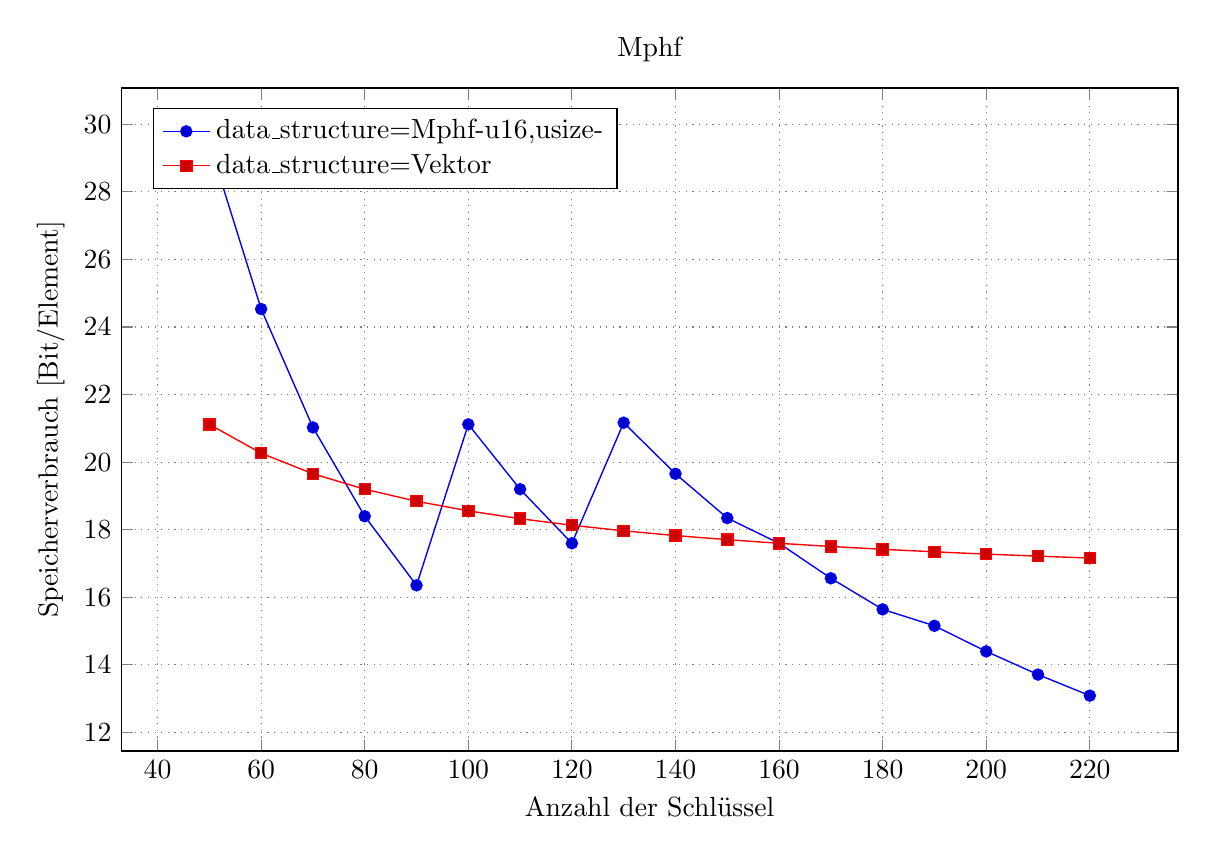
\begin{tikzpicture}
	\begin{axis}[
	title={Mphf},
	xlabel={Anzahl der Schlüssel},
	ylabel={Speicherverbrauch [Bit/Element]},
	]
	
	%% MULTIPLOT(data_structure) SELECT size AS x, size_bytes AS y, MULTIPLOT
	%% FROM mphf WHERE x % 10 == 0 AND x<=220 AND x>40 GROUP BY MULTIPLOT,x ORDER BY MULTIPLOT,x
 \addplot coordinates { (50,29.44) (60,24.5333) (70,21.0286) (80,18.4) (90,16.3556) (100,21.12) (110,19.2) (120,17.6) (130,21.1692) (140,19.6571) (150,18.3467) (160,17.6) (170,16.5647) (180,15.6444) (190,15.1579) (200,14.4) (210,13.7143) (220,13.0909) };
 \addlegendentry{data\_structure=Mphf-u16,usize-};
 \addplot coordinates { (50,21.12) (60,20.2667) (70,19.6571) (80,19.2) (90,18.8444) (100,18.56) (110,18.3273) (120,18.1333) (130,17.9692) (140,17.8286) (150,17.7067) (160,17.6) (170,17.5059) (180,17.4222) (190,17.3474) (200,17.28) (210,17.219) (220,17.1636) };
 \addlegendentry{data\_structure=Vektor};
 
 
	
	\end{axis}
	\end{tikzpicture}
\end{center}




\end{document}

%%%%%%%%%%%%%%%%%%%%%%%%%%%%%%%%%%%%%%%%%%%%%%%%%%%%%%%%%%%%%%%%%%%%%%%%%%%%%%%%
